\subsection{ARCore}
% - ARCore: definition, scope of the library, other applications (FIXME: move to a background section?)
ARCore is an augmented reality framework provided by Google.
The project's roots began in a prototype framework called \enquote{Project Tango} in 2014 and had its first proper release in March 2018 \footnote{https://arstechnica.com/gadgets/2017/08/googles-arcore-brings-augmented-reality-to-millions-of-android-devices/}.
ARCore is available on various platforms, including Android, iOS and the Unity Game Engine \footnote{https://developers.google.com/ar/discover/}.

% - Concepts: session w/ tracking info, anchors, plane detection --> focused on getting a stable "game board"
The core of ARCore is formed by a session which holds the features needed to track the movement of the user's phone as they move the device through three dimensional space.
ARCore will continuously select tracking points based on the images from  the camera and compute the delta to points it found previously.
Based on a set of these points, its main task is to detect and maintain stable planes that can act as a game board for virtual objects.
It is then possible to register "anchors" with the session on the current location of any tracking point or any point on a detected plane.
The position of these anchors will then be updated in the virtual space as ARCore's understanding of the real space changes. \footnote{https://developers.google.com/ar/discover/concepts}

% - our use: getting an idea about the room's dimensions, moving objects in virtual scene believably relative to phone's movement
For Demon GO, we aimed to have a virtual demon fly through the physical space the player is currently in.
As a consequence we had no use for ARCore's main feature of detecting planes, other than them being potential obstacles for collision detection.
Instead, our use of ARCore served to get an estimate about the physical space's dimensions and having the demon move believably relative to the camera's movement.

% - estimating room size: incentivizing turning by defining a "start room" for demon that progressively grows --> assumes user is not pressed against a wall
To estimate the size of the physical space, we first define a small start area of about 2 by 2 by 2 meters around the origin of the ARCore coordinate system, which corresponds to the location of the phone when the session was started, but moved to where ARCore believes the ground to be.
The demon will move quickly to random points within this box, encouraging the player to turn to find the demon again.
This way, we typically receive impressions in all four major directions of the physical space.
ARCore will create tracking points as soon as the camera image changes and provide us with an estimate of their location in virtual space.
We use these estimates to progressively grow the box the demon is allowed to use, such that, in the end, it will ideally be able to roam freely in a box-shaped estimate of the physical space.
We limit the maximum extent of the space relative to the origin to keep the demon close by in open physical spaces.

% - problems w/ room size: abusing tracking points might include outliers that artificially extend the room --> makes game elements inaccessible; fast movement may reduce quality
Two issues arose from this approach: first, tracking points may include outliers that artificially extend the room size.
This will have the most undesired consequence of game elements appearing to penetrate walls while providing X-ray vision to the user and put them effectively out of reach for any user interactions.
Second, the fact that the demon moves quickly in small spaces initially not only encourages turning, but specifically may prompt players to turn quickly.
The quick movement, however, reduces the quality of the camera images and makes it harder for ARCore to compute the delta movement, which in turn also reduces the quality of the understanding of the room's size as it is provided to us by ARCore.

To reduce the impact on gameplay of this issue, we stopped relying on the room dimensions and instead started using only locations where we knew that ARCore had found high quality image features.
The algorithm works as follows: We define four points in all directions around the user in a plus-like shape, all of them 30 meters away and with the lowest possible confidence, which we designate as the best points.
In each frame, we get the tracking point with the highest reported confidence, as reported by ARCore, and remember it as our candidate point.
We then find the best point closest to our candidate and replace the current best, if the candidate's confidence is higher.
When the points are requested by the pipeline, we will first try to fill up points using our best points, if their confidence is higher than a threshold.
Otherwise we, again, fall back to using random points.
Using this method, we managed to get the demon to very stable positions most of the time, while still ensuring that it will not always be in the same corner of the room, where a lot of high quality of high-confidence points were found, as those will keep only replacing their closest best and not affect the other three.

\subsection{Snapshots}
% - every frame is distilled into a "Snapshot" containing pixel data, all tracking points, view-proj-matrices. pixel data is passed on to pipeline
We distill every frame provided by ARCore to a snapshot.
This snapshot contains the pixel data, typically at a resolution of 1080 by 1920 pixels, the position in virtual space of all tracking points currently in the ARCore session and the current view and projection matrices of the virtual camera. See figure \ref{fig:snapshot_data} for a Visualization.
These snapshots are pushed to a queue to which the pipeline of the exploitation subsystem, which runs in a separate thread, can pop from.

\begin{figure}
    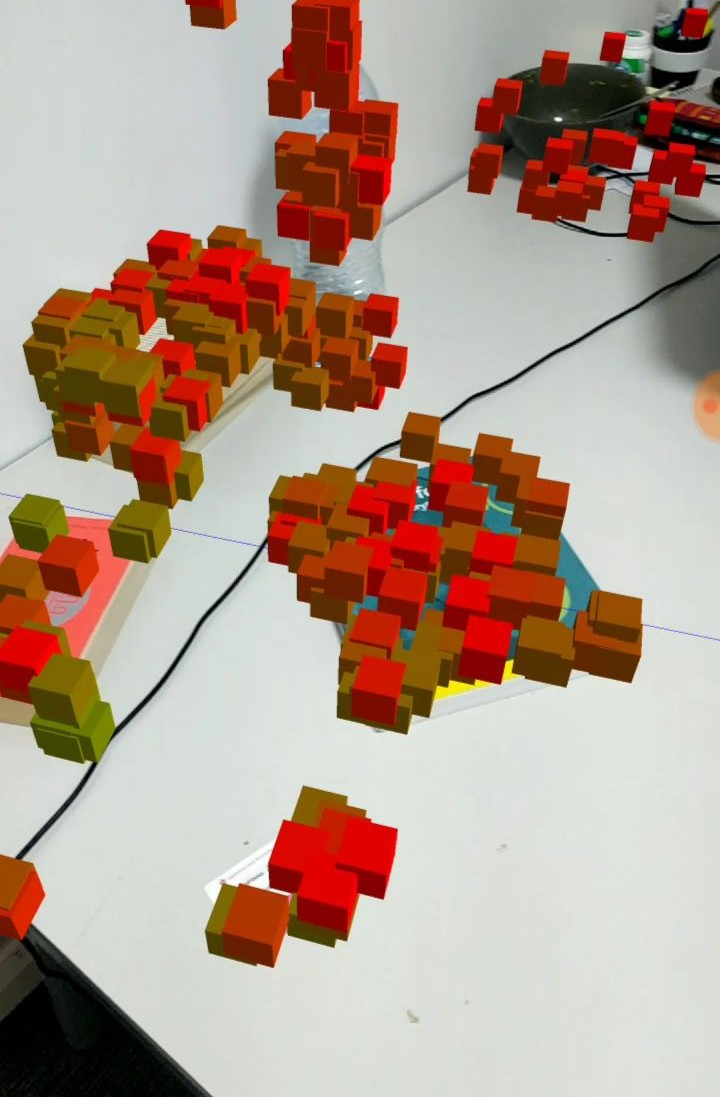
\includegraphics[height=6cm]{graphics/snapshot-points.jpg}
    \caption{Visualization of the information saved in a snapshot. Visible are the pixel data of the image and the subset of tracking points that are saved, symbolized by the cubes. Red cubes report a low confidence, green cubes a high confidence. The confidence information is currently not persisted in the snapshots, but useful for debugging.}
    \label{fig:snapshot_data}
\end{figure}

% - pipeline reports back with 2d PoI
% - challenge: likely won't have depth component for an arbitrary point on image
% - solution: project tracking points to 2d plane, find closest
When the pipeline has established what the points of interest in the picture of a snapshot are, if any, it will instruct the snapshot to map their two dimensional location on the picture back to a three dimensional point in the virtual game space.
Due to the nature of the tracking points only appearing in segments of the picture that contain many features, we do not have a depth component for an arbitrary point on the image.
However, most of the time, we will have multiple tracking points close by, as points of interest are often found in areas with a lot of distinct objects, that is, not just a white wall, but for example characters on a piece of paper or a brand logo.
To solve the problem of lack of depth information, we make the assumption that any point that is as close as possible will suffice for our use case, since the 3D point is only used to direct our demon to the general area of the point of interest, in order to also lure the player to that same point.
As such, we simply project all 3D tracking points onto the 2D plane of our picture using the virtual camera's view-projection and select the corresponding 3D point of the closest point in 2D space as our point of interest in the virtual space.

% - pipeline calls project method, stores best hits for PoI
% - game/AR component later requests best 0-5 PoI from pipeline
% - generates random ones within room at reachable height to make game experience more consistent (i.e. not make game easier in plain rooms)
After projecting its 2D points of interest to 3D points, the pipeline will store these points along with a score.
When the game informs the pipeline that the scanning phase is over and we need to move to the capturing phase, the pipeline will select those points with a highest score and provide them to the game subsystem.
The game subsystem will then select between three and five points for the route of the demon during the capturing phase.
If the pipeline provided too many points, those with a lower score will be discarded.
If too little points were provided, the game subsystem will generate new points by randomly selecting a 3D point in the box that was previously established to be our physical space.
This ensures that the game experience will appear coherent, independent of the output of the exploitation subsystem.
